%%%%%%%%%%%%%%%%%%%%%%%%%%%%%%%%%%%%%%%%%
% Beamer Presentation
% LaTeX Template
% Version 1.0 (10/11/12)
%
% This template has been downloaded from:
% http://www.LaTeXTemplates.com
%
% License:
% CC BY-NC-SA 3.0 (http://creativecommons.org/licenses/by-nc-sa/3.0/)
%
%%%%%%%%%%%%%%%%%%%%%%%%%%%%%%%%%%%%%%%%%

%----------------------------------------------------------------------------------------
%	PACKAGES AND THEMES
%----------------------------------------------------------------------------------------

\documentclass{beamer}

\mode<presentation> {
\usetheme{CambridgeUS}
\usecolortheme{rose}
}

\usepackage[utf8]{inputenc}
\usepackage[russian]{babel}
\usepackage{graphicx}
\usepackage{listings}
\usepackage{inconsolata}
\usepackage{amsmath}
\usepackage{amsfonts}
\usepackage{amssymb}
\usepackage{color}
\usepackage{tikz}
\usepackage{booktabs}
\usepackage{multirow}

\usetikzlibrary{automata,positioning}
\usetikzlibrary{shadows}
\definecolor{bluekeywords}{rgb}{0.13,0.13,1}
\definecolor{greencomments}{rgb}{0,0.5,0}
\definecolor{redstrings}{rgb}{0.9,0,0}

\usepackage{listings}
\lstset{language=[Sharp]C,
    showspaces=false,
    showtabs=false,
    breaklines=true,
    showstringspaces=false,
    breakatwhitespace=true,
    escapeinside={(*@}{@*)},
    commentstyle=\color{greencomments},
    keywordstyle=\color{bluekeywords},
    stringstyle=\color{redstrings},
    basicstyle=\small\ttfamily,
    breaklines=true,
    tabsize=2,
}

\DeclareMathOperator*{\argmax}{argmax} 

\AtBeginSection[]{
    \begin{frame}
    \vfill
    \centering
    \begin{beamercolorbox}[sep=8pt,center,shadow=true,rounded=true]{title}
        \usebeamerfont{title}\insertsectionhead\par%
    \end{beamercolorbox}
    \vfill
    \end{frame}
}

%----------------------------------------------------------------------------------------
%	TITLE PAGE
%----------------------------------------------------------------------------------------

\title[DTW]{Динамическое выравнивание многомерных временных рядов}

\author{Моргачев Г., Смирнов В., Липницкая Т., \\ Руководитель: Гончаров А.}

\institute{Moscow Institute of Physics and Technology}
\date{\today}

\begin{document}

%------------------------------------------------

\begin{frame}
\titlepage 
\end{frame}

%------------------------------------------------

\begin{frame}
\frametitle{Цели исследования}
    \begin{block}{Цель работы}
        Исследовать влияния выбора внутренней функции расстояния на 
        работу алгоритма DTW.
    \end{block}
    \begin{block}{Проблема}
        При обобщении выравнивания временных рядов на многомерный случай остается 
        открытым вопрос опредления расстояния между парами векторов.
    \end{block}
    \begin{block}{Метод решения}
        Получение оптимальной функции расстояния путем проведения эксперимента на 
        задачах поиска паттернов и кластеризации
    \end{block}
\end{frame}
    
%------------------------------------------------

\begin{frame}
\frametitle{Постановка задачи}
    \begin{block}{}
        Есть множество временных рядов $\mathbb{S} \subset \mathbb{R}^{l \times n}$,
         где $l$ \-- количество каналов,\\ $n$ \-- длина ряда. \\
        Задано множество функций расстояния между векторами
        $$\mathrm{R} = \{\rho: \mathbb{R}^n \times \mathbb{R}^n \rightarrow \mathbb{R}^+ \}$$
        $$
            DTW_{\rho}: \mathbb{S} \times \mathbb{S} \rightarrow \mathbb{R}^+ 
        $$
    \end{block}
    \begin{block}{Кластеризация}

        $\forall s_i \in S \subset \mathbb{S}$ задано ${y_i \in \mathbb{Y}}$ \-- множество меток классов.
        Матрица попарных расстояний:
        $$
            D(DTW_\rho(S)) = ||D_{ij}||, \ \ D_{ij} = DTW_\rho(s_i, s_j),\ \ s_i, s_j \in S 
        $$
        Кластеризатор: $f: D \rightarrow Z^N, \ \text{Z \-- множество меток кластеров}$

    \end{block}
\end{frame}

\begin{frame}
    \begin{block}{Функции качества кластеризации}
    \begin{align*}
        Q_1(f(D), S) &= \frac{1}{|Z|}\sum\limits_{z \in Z} \max_y \frac{N_z^y}{N_z}  \\
        Q_2(f(D), S) &= \frac{1}{|Z|}\sum\limits_{z \in Z} \max_y \frac{(N_z^y)^2}{N_z N^y}
    \end{align*}
    \end{block}

    \begin{block}{Поиск паттернов}
        Задан временной ряд $\mathcal{A}$ длинны $n$, содержащий подряды класса $P$. \\
        $P$ \-- временные ряда длины $m \ll n$. \\
        Известны представители класса $P$, необходимо найти участки $\mathcal{A}$,
            соответствующие данному классу. \\
        $T = \{t_1, \dots, t_j \}$ \-- множество начал таких событий. \\
        Участок найден, если пересечение с предполагаемым более $80\%$ от $m$.
    \end{block}
\end{frame}

\begin{frame}
    \begin{block}{Функции качества поиска шаблонов}
        \begin{align*}
            Q(DTW_{\rho}, A, P_k, T) = \dfrac{\sum\limits_{i=1}^j [t_i \-- \text{найден}]}{j}
        \end{align*}
    \end{block}

    \begin{block}{Общая постановка задачи}
        $$
            \rho_i = \argmax_{\rho} Q_i(\rho)
        $$
    \end{block}
\end{frame}
    
%------------------------------------------------
\begin{frame}
\frametitle{Сравнение рядов}
    \begin{block}{Проблемы}
        \begin{itemize}
            \item Растяжение
            \item Сдвиги
        \end{itemize}
    \end{block}
    \begin{figure}
        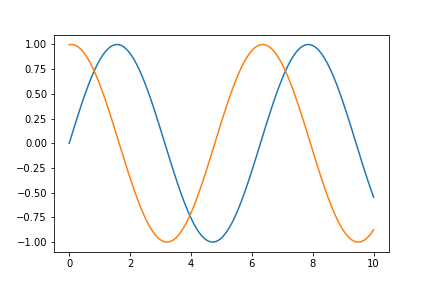
\includegraphics[width=0.6\linewidth]{2}
    \end{figure}
\end{frame}

%------------------------------------------------

\begin{frame}
\frametitle{DTW}
    \begin{block}{DTW}
        \begin{itemize}
            \item Выравнивание рядов друг относительно друга
            \item Позволяет задать функцию расстояния
            \item Использует матрицу попарных расстояний между точками рядов
        \end{itemize} 
    \end{block}
    \begin{figure}
        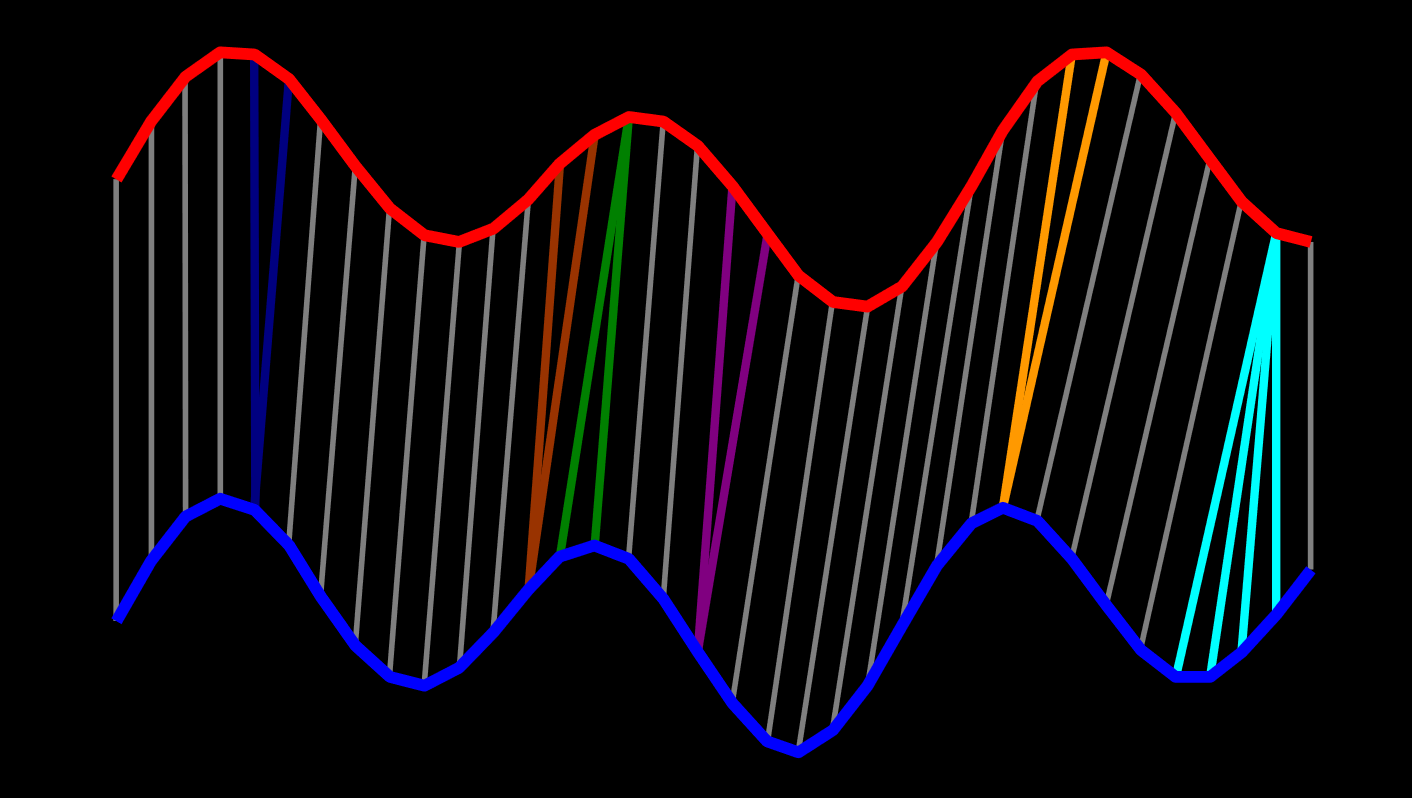
\includegraphics[width=0.6\linewidth]{1}
    \end{figure}
\end{frame}


%------------------------------------------------

\begin{frame}
\frametitle{Многомерное DTW}    
    \begin{block}{Особенность}
        Необходимость выбора функции расстояния между соответственными точками рядов
    \end{block}

    \begin{block}{Постановка задачи}
        Зависимость качества кластеризации временных рядов от выбора функции расстояния между ними
    \end{block}
\end{frame}
        
%------------------------------------------------

\begin{frame}
    \frametitle{Эксперимент}
    \begin{block}{Кластеризация}
        \textbf{Иерархическая} с функциями расстояния между кластерами: 
        \begin{enumerate}
            \item \textit{complete:}  $d(A, B) = \max\limits_{a \in A, b \in B}(dist(a, b))$ 
            \item \textit{weighted:}  $d(A,B) = \dfrac{(dist(S,B) + dist(T,B))}{2}$, где кластер $A = S \cup T$
            \item \textit{weighted:}  $d(u,v) = \sum\limits_{a \in A, b \in B} \dfrac{d(a, b)}{(|A|*|B|)}$ 
        \end{enumerate} 
    \end{block}
\end{frame}
 
\begin{frame}
    \frametitle{Эксперимент}   
    \begin{block}{Данные: класстеризация}
        \begin{itemize}
            \item Размеченные данные ускорений акселерометра телефона: из 6 состояния человека,
                3 канала, разбит по 50 точек.
        \end{itemize}
    \end{block}

    \begin{block}{Данные: поиск паттернов}
        \begin{itemize}
            \item Данные ECG: 4 состояния человека, 3 канала, разбиты на ряды по 206 точек
            \item Написание букв: 20 символов, 3 канала, разбиты по 182 точки 
        \end{itemize}
    \end{block}
\end{frame}
    
%------------------------------------------------

\begin{frame}
    \frametitle{Результаты: поиск паттернов}   
    \begin{center}
        \begin{table}
            \begin{tabular}{c|c *{2}{|*{3}{c}}}  
                \toprule
                  \multirow{2}{*}{$\rho$}& \multirow{2}{*}{average} & 
                            \multicolumn{3}{c|}{characters} & \multicolumn{3}{c}{epi} \\
                \cmidrule(r){3-8}
                                   &  & $Q$ & $t$ & $t_{\text{no optim}}$ & $Q$ & $t$ & $t_{\text{no optim}}$ \\
                \midrule
            \multirow{2}{*}{$L_1$} 
                    & DBA    &   0.857   &   2.123   &    11.767   &   0.744   &   14.335   &    13.064\\
                    & mean   &   0.894   &   2.361   &    11.614   &   0.744   &   13.541   &    13.912\\
            \midrule        
            \multirow{2}{*}{$L_2$} 
                    & DBA    &   0.818   &   1.551   &    11.499   &   0.687   &   12.342   &    13.205\\
                    & mean   &   0.854   &   1.527   &    10.164   &   0.687   &   14.199   &    12.738\\
            \midrule        
            \multirow{2}{*}{ED}
                    & DBA    &   0.08   &   17.511   &    17.511   &   0.172  &   1.620   &    1.620   \\
                    & mean   &   0.09   &   17.645   &    17.645   &    0.172  &   1.540   &    1.540    \\
            \bottomrule
            \end{tabular}
        \end{table}
    \end{center}
\end{frame}


%------------------------------------------------

\begin{frame}
    \frametitle{Результаты: кластеризация}   
    \begin{table}[h]
        \centering
        \begin{tabular}{c|c *{2}{|*{3}{c}}}
            \toprule
            \multirow{2}{*}{$\rho$} & \multirow{2}{*}{$N_{clust}$} & \multicolumn{3}{c|}{$Q_1$} & \multicolumn{3}{c}{$Q_2$} \\
            \cmidrule(r){3-8}
            && \textit{compl.} & \textit{aver.} & \textit{weight.} & \textit{compl.} & \textit{aver.} & \textit{weight.} \\
            \midrule
        \multirow{3}{*}{$L_1$}
                & 24    &   0.506  &   0.585 &    0.638  & 0.273   &  0.376    &   0.449  \\
                & 36    &   0.533  &   0.620 &    0.616  & 0.299   &  0.425    &   0.414  \\
                & 48    &   0.556  &   0.639 &    0.631  & 0.330   &  0.443    &   0.431  \\
        \midrule
        \multirow{3}{*}{$L_2$}
                & 24    &   0.488  &   0.622 &    0.626  & 0.270   &  0.417    &   0.425  \\
                & 36    &   0.498  &   0.646 &    0.643  & 0.270   &  0.455    &   0.449  \\
                & 48    &   0.534  &   0.648 &    0.653  & 0.270   &  0.455    &   0.462  \\
        \bottomrule
        \end{tabular}
    \end{table}

\end{frame}

%------------------------------------------------

\begin{frame}
    \frametitle{Результаты}
    \begin{block}{Выводы}
        
    \end{block}
\end{frame}
    
%------------------------------------------------
\begin{frame}
    \begin{center}
        \Huge Спасибо за внимание!
    \end{center}
\end{frame}

%----------------------------------------------------------------------------------------
\end{document} 